% Created 2025-05-21 Wed 07:54
% Intended LaTeX compiler: pdflatex
\documentclass[a4paper,12pt]{article}
\usepackage[utf8]{inputenc}
\usepackage[T1]{fontenc}
\usepackage{amsmath}
\usepackage{amssymb}
\usepackage{capt-of}
\usepackage{hyperref}
\usepackage{amsthm}
\usepackage{amssymb}
\usepackage{mathtools}
%\documentclass[12pt]{article}
\usepackage{geometry}

\usepackage{amsmath}
\usepackage{amssymb,amsfonts,textcomp}
\usepackage[T1]{fontenc}
\usepackage[utf8]{inputenc}
\usepackage{times} % Times New Roman font
\usepackage{setspace}
\usepackage[pdftex]{graphicx}

\usepackage{hyperref}

% Set line spacing to 1.5
\setstretch{1.5}

\geometry{a4paper, portrait, margin=0.7in, nohead}

\usepackage{titlesec}
\titleformat{\section}[block]{\normalfont\large\bfseries}{\thesection}{1em}{}
\titleformat{\subsection}[block]{\normalfont\large\bfseries}{\thesubsection}{1em}{}

\makeatletter

\newcommand{\student}[1]{\author{#1}}

\newcommand{\group}[1]{\def\@group{#1}}

\newcommand{\prof}[1]{\def\@prof{#1}}
\newcommand{\profdep}[1]{\def\@profdep{#1}}

\newcommand{\labno}[1]{\def\@labno{#1}}

\newcommand{\labtopic}[1]{\title{#1}}

\group{FAF--233}
\prof{Fistic Cristofor}
\profdep{sea, fcim utm}
\labno{3}

%% ox-latex features:
%   !announce-start, !guess-pollyglossia, !guess-babel, !guess-inputenc,
%   engraved-code, caption, maths, image, !announce-end.

% Setup for code blocks [1/2]

\usepackage{fvextra}

\fvset{%
  commandchars=\\\{\},
  highlightcolor=white!95!black!80!blue,
  breaklines=true,
  breaksymbol=\color{white!60!black}\tiny\ensuremath{\hookrightarrow}}

% Make line numbers smaller and grey.
\renewcommand\theFancyVerbLine{\footnotesize\color{black!40!white}\arabic{FancyVerbLine}}

\usepackage{xcolor}

% In case engrave-faces-latex-gen-preamble has not been run.
\providecolor{EfD}{HTML}{f7f7f7}
\providecolor{EFD}{HTML}{28292e}

% Define a Code environment to prettily wrap the fontified code.
\usepackage[breakable,xparse]{tcolorbox}
\providecommand{\codefont}{\footnotesize}
\DeclareTColorBox[]{Code}{o}%
{colback=EfD!98!EFD, colframe=EfD!95!EFD,
  fontupper=\setlength{\fboxsep}{0pt}\codefont,
  colupper=EFD,
  IfNoValueTF={#1}%
  {boxsep=2pt, arc=2.5pt, outer arc=2.5pt,
    boxrule=0.5pt, left=2pt}%
  {boxsep=2.5pt, arc=0pt, outer arc=0pt,
    boxrule=0pt, leftrule=1.5pt, left=0.5pt},
  right=2pt, top=1pt, bottom=0.5pt,
  breakable}

% Support listings with captions
\usepackage{float}
\floatstyle{plain}
\newfloat{listing}{htbp}{lst}
\newcommand{\listingsname}{Listing}
\floatname{listing}{\listingsname}
\newcommand{\listoflistingsname}{List of Listings}
\providecommand{\listoflistings}{\listof{listing}{\listoflistingsname}}


% Setup for code blocks [2/2]: syntax highlighting colors

\newcommand\efstrut{\vrule height 2.1ex depth 0.8ex width 0pt}
\definecolor{EFD}{HTML}{000000}
\definecolor{EfD}{HTML}{ffffff}
\newcommand{\EFD}[1]{\textcolor{EFD}{#1}} % default
\definecolor{EFh}{HTML}{7f7f7f}
\newcommand{\EFh}[1]{\textcolor{EFh}{#1}} % shadow
\definecolor{EFsc}{HTML}{228b22}
\newcommand{\EFsc}[1]{\textcolor{EFsc}{\textbf{#1}}} % success
\definecolor{EFw}{HTML}{ff8e00}
\newcommand{\EFw}[1]{\textcolor{EFw}{\textbf{#1}}} % warning
\definecolor{EFe}{HTML}{ff0000}
\newcommand{\EFe}[1]{\textcolor{EFe}{\textbf{#1}}} % error
\definecolor{EFc}{HTML}{b22222}
\newcommand{\EFc}[1]{\textcolor{EFc}{#1}} % font-lock-comment-face
\definecolor{EFcd}{HTML}{b22222}
\newcommand{\EFcd}[1]{\textcolor{EFcd}{#1}} % font-lock-comment-delimiter-face
\definecolor{EFs}{HTML}{8b2252}
\newcommand{\EFs}[1]{\textcolor{EFs}{#1}} % font-lock-string-face
\definecolor{EFd}{HTML}{8b2252}
\newcommand{\EFd}[1]{\textcolor{EFd}{#1}} % font-lock-doc-face
\definecolor{EFm}{HTML}{008b8b}
\newcommand{\EFm}[1]{\textcolor{EFm}{#1}} % font-lock-doc-markup-face
\definecolor{EFk}{HTML}{9370db}
\newcommand{\EFk}[1]{\textcolor{EFk}{#1}} % font-lock-keyword-face
\definecolor{EFb}{HTML}{483d8b}
\newcommand{\EFb}[1]{\textcolor{EFb}{#1}} % font-lock-builtin-face
\definecolor{EFf}{HTML}{0000ff}
\newcommand{\EFf}[1]{\textcolor{EFf}{#1}} % font-lock-function-name-face
\definecolor{EFv}{HTML}{a0522d}
\newcommand{\EFv}[1]{\textcolor{EFv}{#1}} % font-lock-variable-name-face
\definecolor{EFt}{HTML}{228b22}
\newcommand{\EFt}[1]{\textcolor{EFt}{#1}} % font-lock-type-face
\definecolor{EFo}{HTML}{008b8b}
\newcommand{\EFo}[1]{\textcolor{EFo}{#1}} % font-lock-constant-face
\definecolor{EFwr}{HTML}{ff0000}
\newcommand{\EFwr}[1]{\textcolor{EFwr}{\textbf{#1}}} % font-lock-warning-face
\newcommand{\EFnc}[1]{#1} % font-lock-negation-char-face
\definecolor{EFpp}{HTML}{483d8b}
\newcommand{\EFpp}[1]{\textcolor{EFpp}{#1}} % font-lock-preprocessor-face
\newcommand{\EFrc}[1]{\textbf{#1}} % font-lock-regexp-grouping-construct
\newcommand{\EFrb}[1]{\textbf{#1}} % font-lock-regexp-grouping-backslash
\newcommand{\EFob}[1]{#1} % org-block
\definecolor{EFhn}{HTML}{008b8b}
\newcommand{\EFhn}[1]{\textcolor{EFhn}{#1}} % highlight-numbers-number
\definecolor{EFhq}{HTML}{9370db}
\newcommand{\EFhq}[1]{\textcolor{EFhq}{#1}} % highlight-quoted-quote
\definecolor{EFhs}{HTML}{008b8b}
\newcommand{\EFhs}[1]{\textcolor{EFhs}{#1}} % highlight-quoted-symbol
\definecolor{EFrda}{HTML}{707183}
\newcommand{\EFrda}[1]{\textcolor{EFrda}{#1}} % rainbow-delimiters-depth-1-face
\definecolor{EFrdb}{HTML}{7388d6}
\newcommand{\EFrdb}[1]{\textcolor{EFrdb}{#1}} % rainbow-delimiters-depth-2-face
\definecolor{EFrdc}{HTML}{909183}
\newcommand{\EFrdc}[1]{\textcolor{EFrdc}{#1}} % rainbow-delimiters-depth-3-face
\definecolor{EFrdd}{HTML}{709870}
\newcommand{\EFrdd}[1]{\textcolor{EFrdd}{#1}} % rainbow-delimiters-depth-4-face
\definecolor{EFrde}{HTML}{907373}
\newcommand{\EFrde}[1]{\textcolor{EFrde}{#1}} % rainbow-delimiters-depth-5-face
\definecolor{EFrdf}{HTML}{6276ba}
\newcommand{\EFrdf}[1]{\textcolor{EFrdf}{#1}} % rainbow-delimiters-depth-6-face
\definecolor{EFrdg}{HTML}{858580}
\newcommand{\EFrdg}[1]{\textcolor{EFrdg}{#1}} % rainbow-delimiters-depth-7-face
\definecolor{EFrdh}{HTML}{80a880}
\newcommand{\EFrdh}[1]{\textcolor{EFrdh}{#1}} % rainbow-delimiters-depth-8-face
\definecolor{EFrdi}{HTML}{887070}
\newcommand{\EFrdi}[1]{\textcolor{EFrdi}{#1}} % rainbow-delimiters-depth-9-face


\usepackage{capt-of}

\usepackage{amsmath}
\usepackage{amssymb}

\usepackage{graphicx}

%% end ox-latex features


\author{Andrei Chicu}
\date{\today}
\title{Study and empirical analysis of algorithms: Depth First Search (DFS), Breadth First Search (BFS)}
\hypersetup{
 pdfauthor={Andrei Chicu},
 pdftitle={Study and empirical analysis of algorithms: Depth First Search (DFS), Breadth First Search (BFS)},
 pdfkeywords={},
 pdfsubject={},
 pdfcreator={Emacs 30.1 (Org mode 9.8-pre)},
 pdflang={English}}
\begin{document}

\makeatletter
\begin{titlepage}
\centering


\includegraphics[height=2cm]{utm_logo.png}

\bfseries
\textsc{Ministry of Education and Research of Republic of Moldova} \\
\textsc{Technical University of Moldova} \\
\textsc{Faculty of Computers, Informatics and Microelectronics} \\
\textsc{Department of Software and Automation Engineering} \\
\mdseries

\vfill

\textsc{\Large Analysis of Algorithms} \\
\textsc{\large Laboratory work \#\@labno}\\[0.5cm]

\vspace{12pt}
\newcommand{\HRule}{\rule{\linewidth}{0.5mm}}
\HRule \\[0.2cm]
{ \LARGE \bfseries \@title }\\[0.4cm]
\HRule
\vfill

\begin{minipage}[t]{0.4\textwidth}
\begin{flushleft} \large
\emph{Author:} \\
\@author\\                        
std. gr. \@group
\end{flushleft}
\end{minipage}
~
\begin{minipage}[t]{0.4\textwidth}
\raggedleft \large
\emph{Verified:} \\
\@prof \\
Department of \textsc{\@profdep}
\end{minipage}\\[3cm]
\vfill

Chișinău, 2025
\end{titlepage}
\makeatother
\setcounter{page}{2}
\section{Analysis of Algorithms}
\label{sec:orgcb8df83}
github url: \url{https://github.com/andyp1xe1/aa_labs/tree/main/lab3}
\subsection{Objective}
\label{sec:org6b96727}
The objective of this laboratory work is to implement and analyze two fundamental graph traversal algorithms: Depth First Search (DFS) and Breadth First Search (BFS). The analysis aims to compare their performance across various graph types and sizes to understand their efficiency characteristics, time complexity behavior, and practical applications in different graph scenarios.
\subsection{Tasks}
\label{sec:org719c51f}
\begin{enumerate}
\item Implement the algorithms listed above in a programming language
\item Establish the properties of the input data against which the analysis is performed
\item Choose metrics for comparing algorithms
\item Perform empirical analysis of the proposed algorithms
\item Make a graphical presentation of the data obtained
\item Make a conclusion on the work done.
\end{enumerate}
\subsection{Theoretical Notes}
\label{sec:orgb0e5ee2}

This lab explores various graph algorithms and their applications. Below, we discuss the different types of graphs used in our implementations and analyses.

A graph G is a pair (V, E) where V is a set of vertices (nodes) and E is a set of edges connecting these vertices. In this laboratory work, we focus on directed weighted graphs represented using adjacency lists.
\subsubsection{Types of Graphs}
\label{sec:orgf84a46a}
In this laboratory, we analyze the following types of graphs:
\begin{enumerate}
\item Complete Graph
\label{sec:org5c2e3f4}
Every vertex is connected to every other vertex, resulting in |V|(|V|-1) edges in a directed graph.

\begin{center}
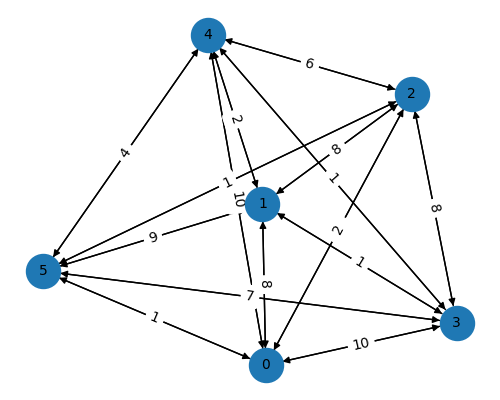
\includegraphics[width=.9\linewidth]{example_complete.png}
\label{orgb8750ea}
\end{center}
\item Dense Graph
\label{sec:orge721fa7}
Has approximately 80\% of the maximum possible edges.

\begin{center}
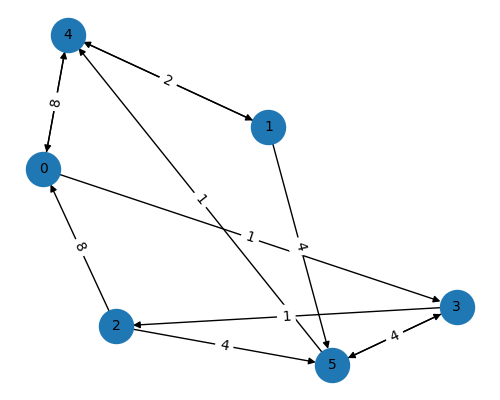
\includegraphics[width=.9\linewidth]{example_dense.png}
\label{orgbeee645}
\end{center}
\item Sparse Graph
\label{sec:orgb8611be}
Contains relatively few edges, approximately 2|V| edges.

\begin{center}
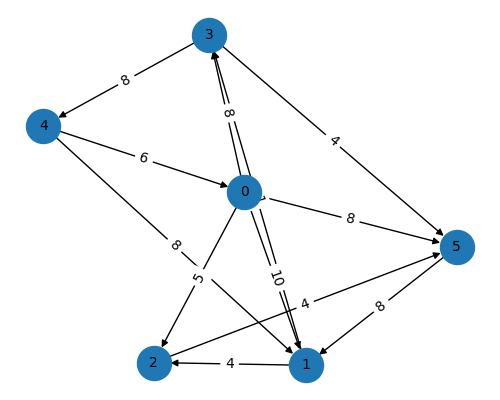
\includegraphics[width=.9\linewidth]{example_sparse.png}
\label{org1f17085}
\end{center}
\item Tree Graph
\label{sec:org2ac6a4e}
Connected acyclic graph with exactly |V|-1 edges.

\begin{center}
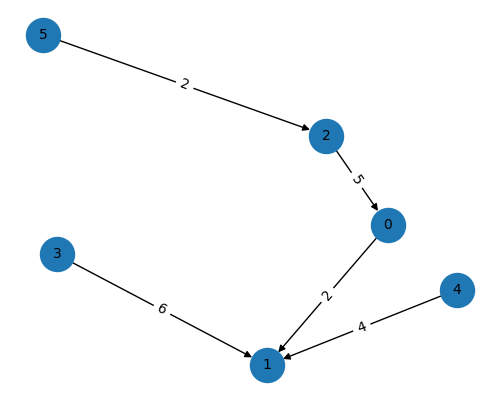
\includegraphics[width=.9\linewidth]{example_tree.png}
\label{org80aebf9}
\end{center}
\item Connected Graph
\label{sec:org36c7aae}
There exists a path between any pair of vertices.

\begin{center}
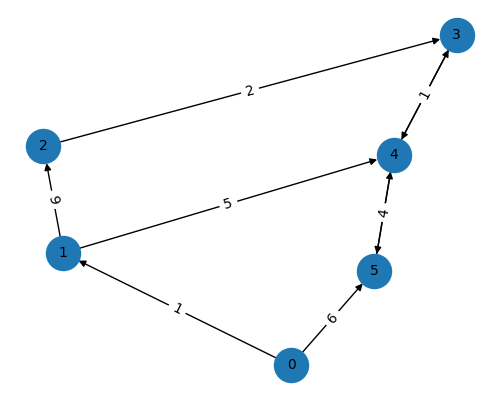
\includegraphics[width=.9\linewidth]{example_connected.png}
\label{org4663983}
\end{center}
\item Cyclic Graph
\label{sec:org2d9021f}
Contains at least one cycle (a path that starts and ends at the same vertex).

\begin{center}
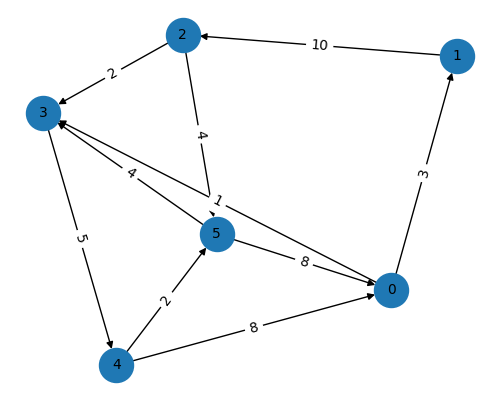
\includegraphics[width=.9\linewidth]{example_cyclic.png}
\label{org63278a1}
\end{center}
\item Acyclic Graph
\label{sec:orgd3bae4e}
Contains no cycles (DAG - Directed Acyclic Graph).

\begin{center}
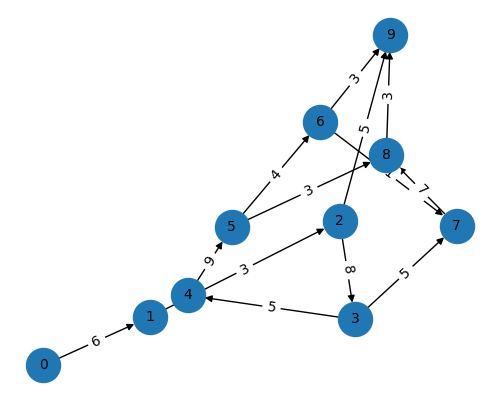
\includegraphics[width=.9\linewidth]{example_acyclic.png}
\label{org13915e7}
\end{center}
\item Grid Graph
\label{sec:orga8ecef2}
Vertices arranged in a grid-like structure with connections primarily to adjacent nodes.

\begin{center}
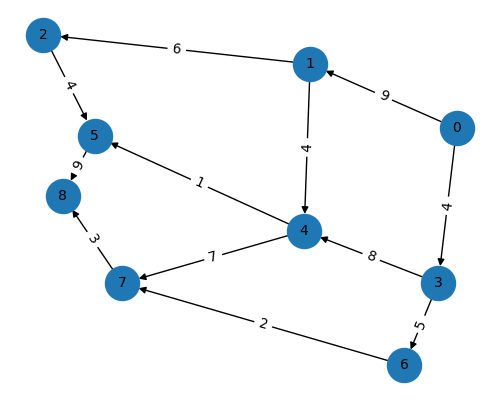
\includegraphics[width=.9\linewidth]{example_grid.png}
\label{orgce13744}
\end{center}
\end{enumerate}
\subsubsection{Depth First Search (DFS)}
\label{sec:orge877121}
DFS is a graph traversal algorithm that explores as far as possible along each branch before backtracking. The algorithm works as follows:
\begin{enumerate}
\item Start at a designated source vertex
\item Explore the first neighbor of the current vertex
\item Continue this process recursively for each unexplored neighbor
\item Backtrack when a vertex has no unexplored neighbors
\item Continue until all reachable vertices have been visited
\end{enumerate}

DFS uses a stack data structure (implicitly through recursion in many implementations) to keep track of vertices.
\subsubsection{Breadth First Search (BFS)}
\label{sec:orgd2fdb2a}
BFS explores all neighbors at the current depth level before moving to vertices at the next depth level:
\begin{enumerate}
\item Start at a designated source vertex
\item Explore all immediate neighbors of the source
\item For each of those neighbors, explore their unexplored neighbors
\item Continue level by level until all reachable vertices have been visited
\end{enumerate}

BFS uses a queue data structure to keep track of vertices to be explored.
\subsection{Comparison Metric}
\label{sec:org5b05c47}
For this empirical analysis, we measure the following metrics:

\begin{enumerate}
\item \textbf{\textbf{Execution Time}}: The primary metric is the actual execution time in seconds for each algorithm across different graph types and sizes. This provides an empirical measure of the algorithm's efficiency.

\item \textbf{\textbf{Visited Nodes}}: The total number of nodes visited during the traversal. In most cases, this will be all reachable nodes from the starting vertex.

\item \textbf{\textbf{Memory Usage}}: Indirectly measured by observing the maximum size of the data structures used (stack for DFS, queue for BFS).
\end{enumerate}

The algorithms are evaluated on various graph types with sizes ranging from 100 to 2500/10,000 vertices to observe how they scale with input size.

\begin{Code}
\begin{Verbatim}
\color{EFD}\EFv{sizes} \textcolor[HTML]{000000}{=} [100, 200, 500, 1000, 2000, 2500]
\EFv{big\_sizes} \textcolor[HTML]{000000}{=} [200, 500, 1000, 2000, 2500, 3000, 3500, 4000, 5000, 6000, 7000, 8000, 9000, 10\_000]
\end{Verbatim}
\end{Code}

For each graph type and size, algorithms were executed with 5 repetitions to account for system variability and provide statistical robustness. This approach allows us to:

\begin{itemize}
\item Calculate mean execution times for more reliable performance comparison
\item Determine standard deviation to assess result consistency and reliability
\item Identify potential outliers or anomalous behavior in specific test cases
\end{itemize}

The error bars in the plots represent the standard deviation across these repetitions, providing a visual indication of measurement variability.
\subsection{Input Format}
\label{sec:orge7d2f47}
In this laboratory work, graphs are represented using adjacency lists implemented as nested Python dictionaries. Each vertex is a key in the outer dictionary, and its value is another dictionary mapping neighboring vertex IDs to edge weights.

The testing framework generates graphs of various types and sizes, then executes both DFS and BFS algorithms on them, measuring the execution time.

Example input graph structure:
\begin{Code}
\begin{Verbatim}
\color{EFD}\EFv{graph} \textcolor[HTML]{000000}{=} \{
    \EFs{'0'}: \{\EFs{'1'}: 5, \EFs{'2'}: 3\},
    \EFs{'1'}: \{\EFs{'3'}: 2, \EFs{'4'}: 4\},
    \EFs{'2'}: \{\},
    \EFs{'3'}: \{\},
    \EFs{'4'}: \{\EFs{'2'}: 1\}
\}
\end{Verbatim}
\end{Code}

In this representation:
\begin{itemize}
\item Vertex '0' has edges to vertices '1' (weight 5) and '2' (weight 3)
\item Vertex '1' has edges to vertices '3' (weight 2) and '4' (weight 4)
\item Vertices '2' and '3' have no outgoing edges
\item Vertex '4' has an edge to vertex '2' (weight 1)
\end{itemize}

All graphs are generated with the functions provided in the uploaded code, with vertices labeled as strings from '0' to 'n-1' and edge weights ranging from 1 to 10.
\section{Implementation}
\label{sec:org1ac15dd}
\subsection{Depth First Search}
\label{sec:orgfe46ea9}
Depth First Search (DFS) is implemented recursively, exploring one path as deeply as possible before backtracking. The algorithm maintains a set of visited vertices to avoid cycles and infinite recursion.

\begin{listing}[htbp]
\begin{Code}
\begin{Verbatim}
\color{EFD}\EFk{def} \EFf{dfs}(graph, start, visited\textcolor[HTML]{000000}{=}\EFo{None}, proc\textcolor[HTML]{000000}{=}\EFo{None}):
    \EFd{"""
    Depth-First Search algorithm implementation.

    Args:
        graph (dict): Adjacency list representation of the graph.
        start (str): Starting vertex.

    Returns:
        list: Order of vertices visited.
    """}
    \EFk{if} visited \EFk{is} \EFo{None}:
        \EFv{visited} \textcolor[HTML]{000000}{=} \EFb{set}()
    \EFk{if} proc \EFk{is} \EFo{None}:
        \EFv{proc} \textcolor[HTML]{000000}{=} []

    visited.add(start)

    \EFk{for} neighbor, weight \EFk{in} graph[start].items():
        \EFk{if} neighbor \EFk{not} \EFk{in} visited:
            proc.append((start, neighbor, weight))
            dfs(graph, neighbor, visited, proc)
    \EFk{return} proc
\end{Verbatim}
\end{Code}
\caption{\label{lst:org46ace5f}Implementation of Depth First Search}
\end{listing}
\subsection{Breadth First Search}
\label{sec:org426d30d}
Breadth First Search (BFS) uses a queue to visit vertices in level order, exploring all neighbors of the current vertex before moving to the next level. Similar to DFS, it maintains a visited set to avoid revisiting vertices.

\begin{listing}[htbp]
\begin{Code}
\begin{Verbatim}
\color{EFD}\EFk{import} collections

\EFk{def} \EFf{bfs}(graph, root):
    \EFd{"""
    Breadth-First Search algorithm implementation.

    Args:
        graph (dict): Adjacency list representation of the graph.
        start (str): Starting vertex.

    Returns:
        list: Order of vertices visited.
    """}
    \EFv{visited} \textcolor[HTML]{000000}{=} \EFb{set}()
    \EFv{queue} \textcolor[HTML]{000000}{=} collections.deque([root])
    visited.add(root)
    \EFv{proc} \textcolor[HTML]{000000}{=} []

    \EFk{while} queue:
        \EFv{vertex} \textcolor[HTML]{000000}{=} queue.popleft()

        \EFk{for} neighbor, weight \EFk{in} graph[vertex].items():
            \EFk{if} neighbor \EFk{not} \EFk{in} visited:
                visited.add(neighbor)
                queue.append(neighbor)
                proc.append((vertex, neighbor, weight))
    \EFk{return} proc
\end{Verbatim}
\end{Code}
\caption{\label{lst:orgfe8927a}Implementation of Breadth First Search}
\end{listing}
\section{Results}
\label{sec:org72c0b3e}
\subsection{Complete Graph}
\label{sec:org0b8a883}
\begin{center}
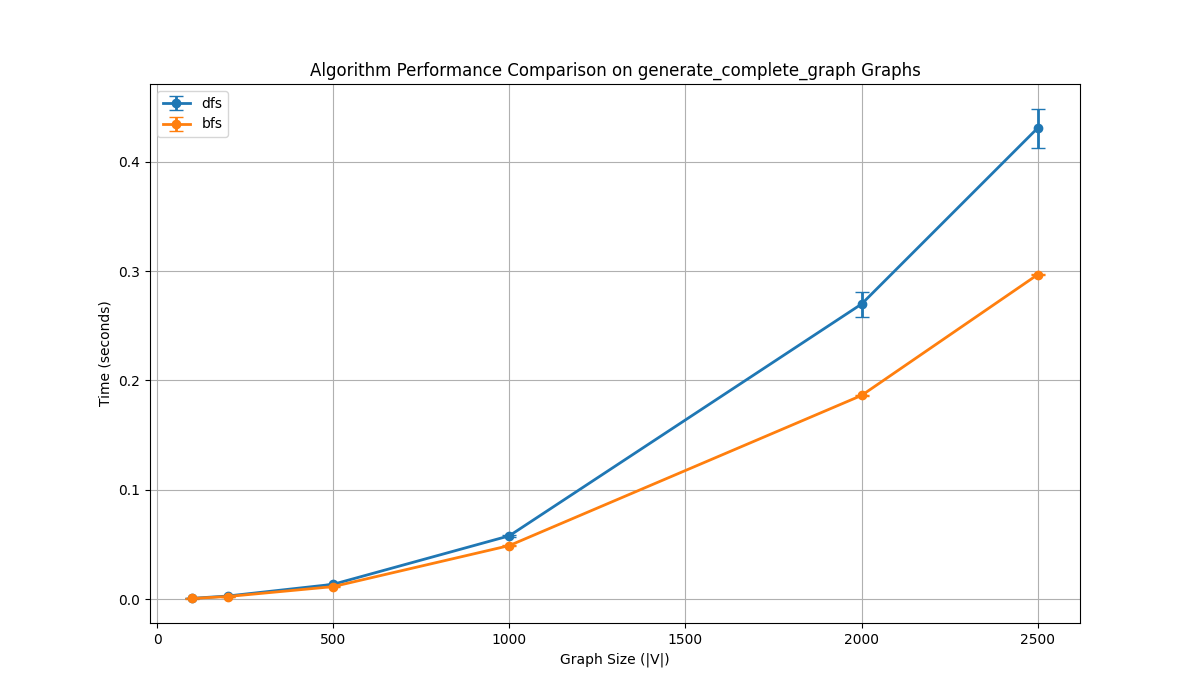
\includegraphics[width=.9\linewidth]{dfs_complete.png}
\label{orgd7dd3c1}
\end{center}
Both algorithms show a clear polynomial growth pattern as the graph size increases, consistent with their O(V+E) complexity where E = O(V²) for complete graphs.

DFS consistently demonstrates higher execution times compared to BFS, with the gap widening as graph size increases. At 2500 vertices, DFS takes approximately 0.43 seconds while BFS requires around 0.30 seconds.

The performance difference is likely due to the recursive implementation of DFS versus the iterative implementation of BFS, which incurs additional function call overhead.

Standard deviation is relatively small for both algorithms, indicating consistent performance across repetitions.
\subsection{Dense Graph}
\label{sec:org010d6ba}
\begin{center}
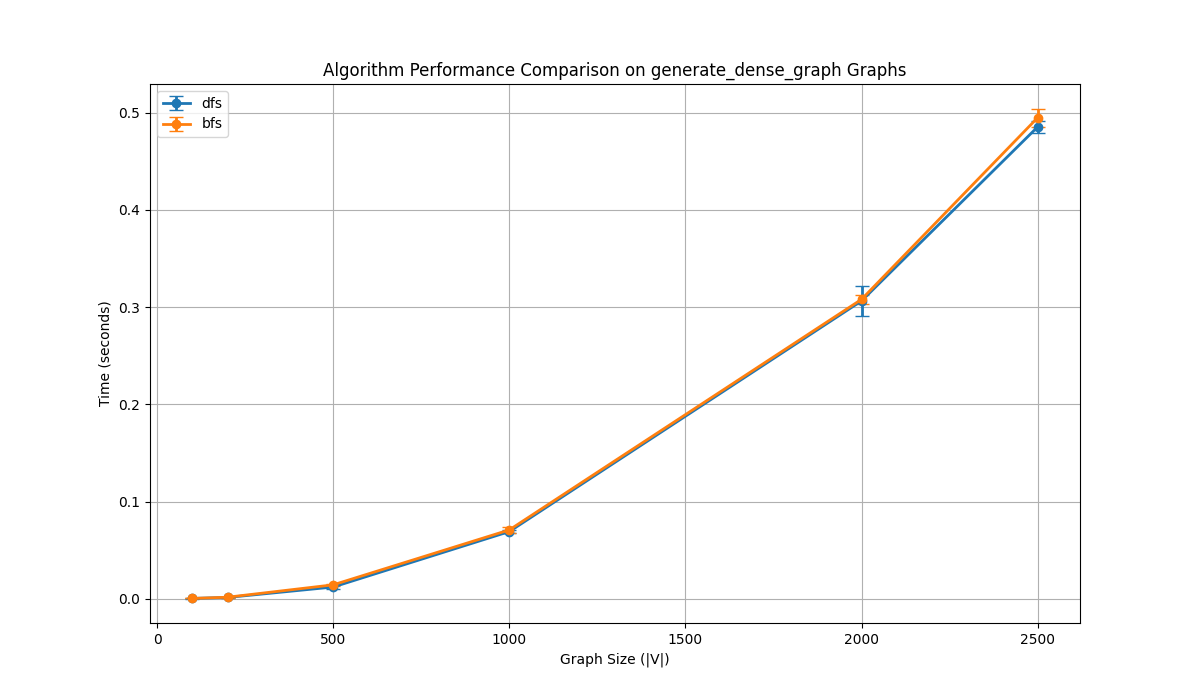
\includegraphics[width=.9\linewidth]{dfs_dense.png}
\label{org1c44216}
\end{center}

In dense graphs (approximately 80\% of maximum possible edges), both algorithms show nearly identical performance profiles.

The execution time growth is polynomial, matching the theoretical expectation for graphs where E ≈ O(V²).

Unlike in complete graphs, the performance difference between DFS and BFS is minimal, suggesting that the overhead of recursion in DFS is offset by other factors in dense but not complete graphs.

The execution times reach approximately 0.5 seconds at 2500 vertices for both algorithms.
Low standard deviation values indicate high consistency in measurement.
\subsection{Sparse Graph}
\label{sec:org1658d8e}
\begin{center}
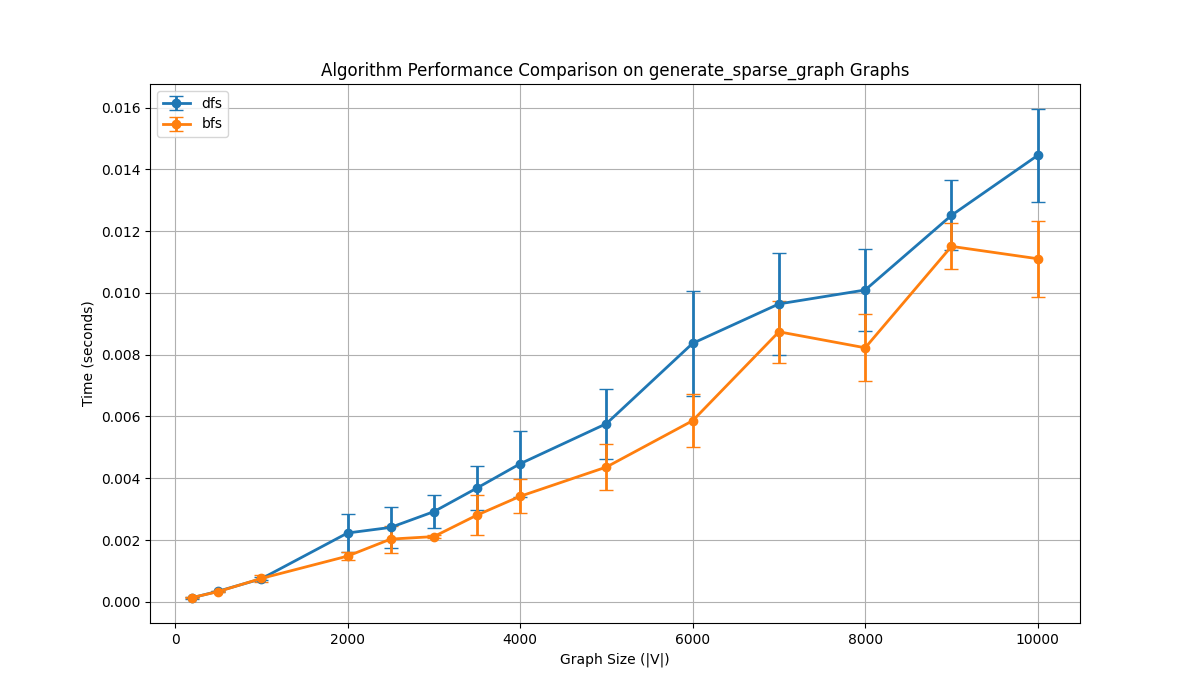
\includegraphics[width=.9\linewidth]{dfs_sparse.png}
\label{orgb0f7cab}
\end{center}

For sparse graphs (with approximately 2|V| edges), both algorithms exhibit a more linear growth pattern, consistent with their theoretical O(V+E) complexity where E = O(V).

DFS consistently performs worse than BFS across all graph sizes, with the gap becoming more pronounced as the graph size increases.

At 10,000 vertices, DFS requires approximately 0.014 seconds while BFS takes around 0.011 seconds.

The standard deviation is relatively higher compared to other graph types, particularly for larger graph sizes, indicating some variability in performance measurements.

The performance advantage of BFS may be attributed to its level-by-level exploration, which could be more efficient in sparse graphs where most paths are relatively long.
\subsection{Tree Graph}
\label{sec:orgded6b34}
\begin{center}
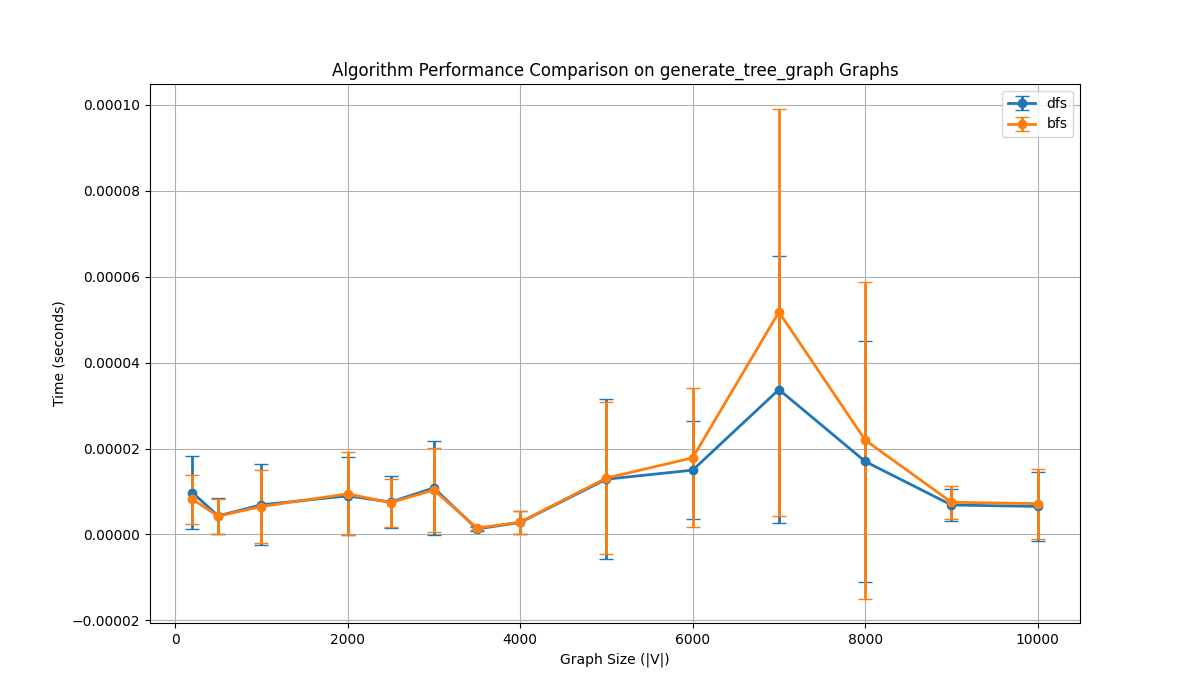
\includegraphics[width=.9\linewidth]{dfs_tree.png}
\label{org5c77c7b}
\end{center}

Tree graphs show the most unusual performance pattern among all tested graph types.

The execution times are extremely small (in the order of 10⁻⁵ seconds) even for large graphs with up to 10,000 vertices.

There is no clear trend in performance as graph size increases, with some larger graphs actually showing faster execution times than smaller ones.

The standard deviation is proportionally very large, often comparable to or exceeding the mean execution time.
The unusual behavior might be attributed to:
\begin{itemize}
\item Highly efficient traversal of tree structures
\item Caching effects becoming significant at these small time scales
\item System timing resolution limitations at microsecond scales
\end{itemize}

The negative values on the y-axis are likely visualization artifacts due to error bars extending below zero.
\subsection{Connected Graph}
\label{sec:orgaf84068}
\begin{center}
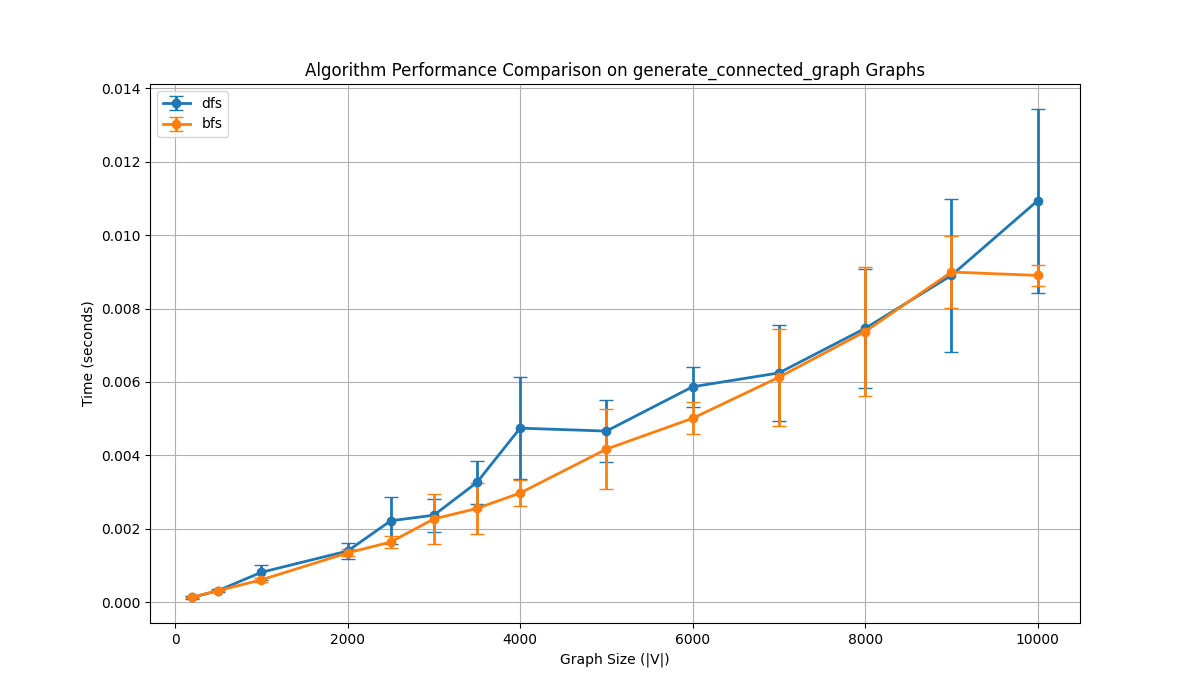
\includegraphics[width=.9\linewidth]{dfs_connected.png}
\label{orgef1528f}
\end{center}

Both algorithms show a linear growth pattern, consistent with O(V+E) complexity when E is proportional to V.

DFS performs slightly worse than BFS at larger graph sizes, but the difference is minimal compared to other graph types.

At 10,000 vertices, DFS takes approximately 0.011 seconds while BFS requires around 0.009 seconds.

The standard deviation increases with graph size but remains relatively consistent between the two algorithms.

The minimal performance difference suggests that both algorithms are well-suited for connected graphs with moderate edge density.
\subsection{Cyclic Graph}
\label{sec:org7ffd6e1}
\begin{center}
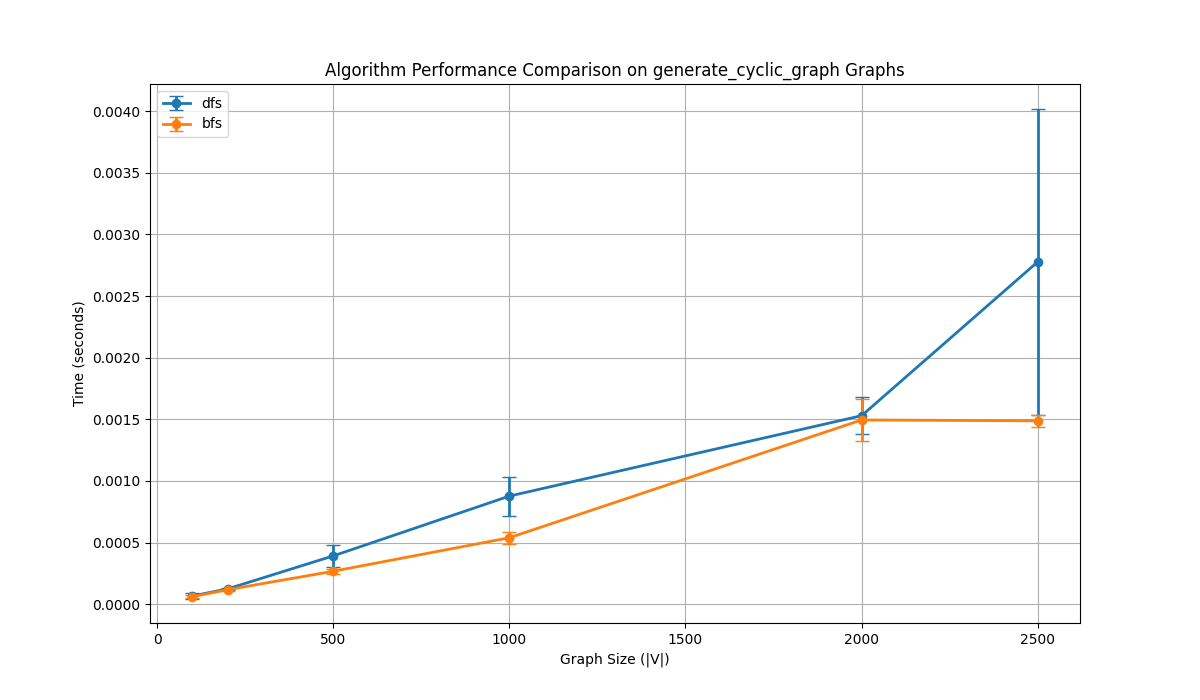
\includegraphics[width=.9\linewidth]{dfs_cyclic.png}
\label{orgd373a87}
\end{center}

Both algorithms show a linear growth pattern up to 2000 vertices, after which BFS maintains linear growth while DFS begins to exhibit slightly faster growth.

At 2500 vertices, DFS takes approximately 0.0027 seconds while BFS requires around 0.0015 seconds.

BFS appears to handle cycles more efficiently than DFS, possibly because it avoids the deep recursion that can occur when DFS encounters cycles.

The standard deviation is moderate and increases with graph size, indicating reasonable measurement consistency.
\subsection{Acyclic Graph}
\label{sec:org4e7515a}
\begin{center}
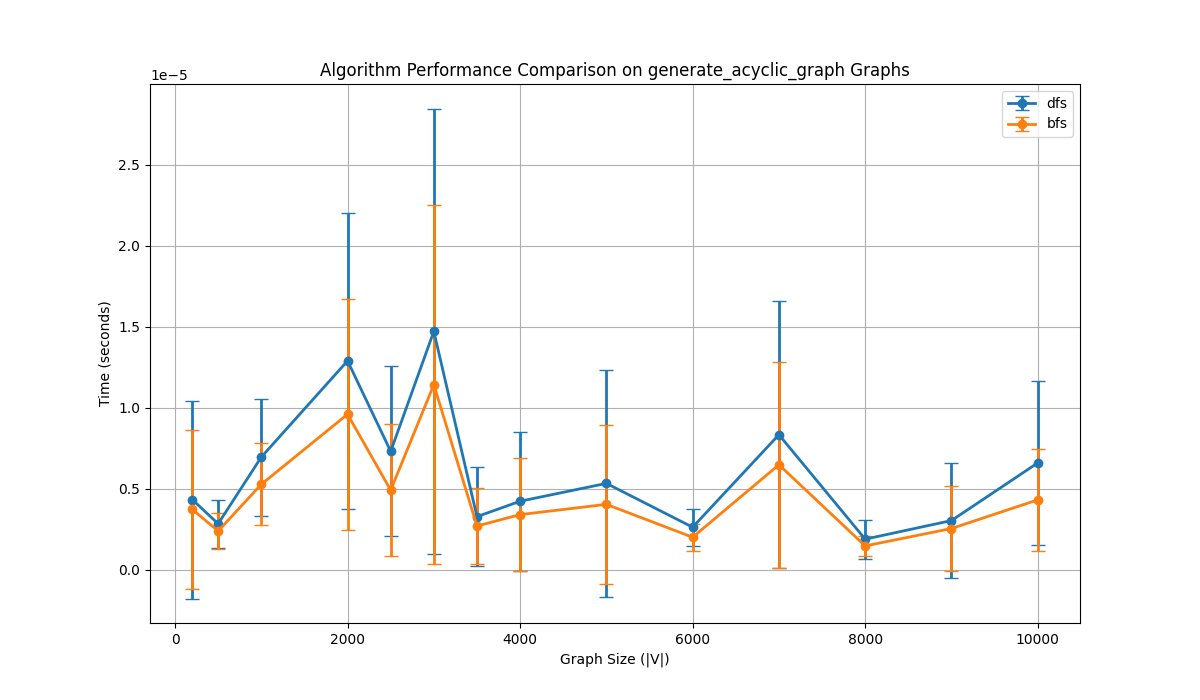
\includegraphics[width=.9\linewidth]{dfs_acyclic.png}
\label{org676f13e}
\end{center}

The acyclic graph tests show the most erratic behavior among all graph types, with significant fluctuations in execution time across different graph sizes.

Despite the fluctuations, there is a general upward trend in execution time as graph size increases.

BFS generally outperforms DFS, particularly at larger graph sizes.
The error bars are exceptionally large, indicating high variability across repetitions.

The erratic behavior might be attributed to:
\begin{itemize}
\item Specific topological characteristics of the generated acyclic graphs
\item Memory access patterns that vary significantly between runs
\item System scheduling effects becoming more pronounced
\end{itemize}
\subsection{Grid Graph}
\label{sec:orgf7c8b82}
\begin{center}
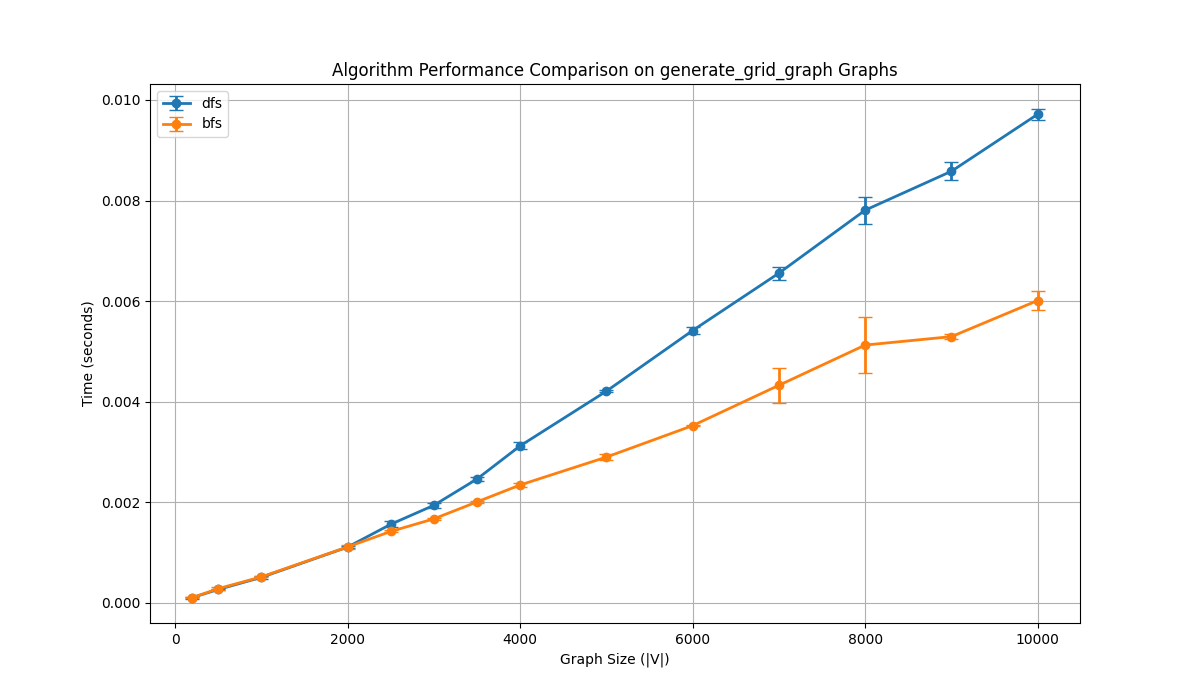
\includegraphics[width=.9\linewidth]{dfs_grid.png}
\label{org5b59c1c}
\end{center}

Grid graphs show one of the clearest performance differences between DFS and BFS.

Both algorithms exhibit linear growth with graph size, but DFS shows a steeper slope.

At 10,000 vertices, DFS requires approximately 0.0097 seconds while BFS takes around 0.006 seconds.

The performance gap widens consistently as graph size increases, with BFS maintaining a roughly 40\% advantage at the largest sizes.

The standard deviation is small relative to the mean values, indicating consistent measurements.

BFS's advantage in grid graphs is likely due to its level-by-level exploration pattern, which aligns well with the regular structure of grid graphs.
\section{Conclusions}
\label{sec:org35dbe9c}

This laboratory work demonstrates that while DFS and BFS have the same theoretical time complexity (O(V+E)), their practical performance can vary based on graph structure and implementation details. The choice between these algorithms should consider not only execution time but also the specific requirements of the application, such as path characteristics, memory constraints, and the expected graph structure.

The empirical analysis confirms that while DFS and BFS share the same theoretical time complexity of O(V+E), their practical performance characteristics differ significantly depending on graph structure

BFS is generally more efficient across most graph types, particularly for grid structures and large graphs.
The performance advantage of BFS becomes more pronounced as graph size increases. For complete graphs and some specialized applications where depth-priority is beneficial, DFS may still be appropriate.

The recursive implementation of DFS introduces overhead that impacts real-world performance. An iterative implementation of DFS might reduce this gap. The choice between recursive and iterative implementations represents a trade-off between code clarity and performance.

Most graph types show consistent performance across repetitions, as evidenced by relatively small standard deviations. Tree graphs and acyclic graphs show higher variability, suggesting that performance for these specific structures may be more sensitive to system conditions.

Both algorithms scale according to theoretical predictions based on the relationship between vertices and edges. The practical growth rate is highly dependent on graph structure and edge density

These findings demonstrate the importance of empirical analysis to complement theoretical complexity analysis, as implementation details and structural characteristics can significantly impact real-world algorithm performance.
\end{document}
